% ===================================================================
% Topic1ExplanationsPart1 — pages 23–34
% Topic 1-6 Questions 1–4, Topic 1-7 Question 1, Topic 1-8 Questions 1–4
% ===================================================================

\lesson{Lesson 1-6: Multiply Integers}

\noindent Before Questions 3 and 4, remember the order-of-operations rule called \textbf{PEMDAS}.

\begin{words}
  \item \textbf{P} means \term{Parentheses}: do work inside ( ) first.
  \item \textbf{E} means \term{Exponents}: do powers like $5^{2}$ next.
  \item \textbf{MD} means \term{Multiply}and \term{Divide}: left to right.
  \item \textbf{AS} means \term{Add}and \term{Subtract}: left to right last.
\end{words}

\question{Question 1}

\blockhead{Question}
\noindent A hiker begins at sea level, 0 feet, and descends into a canyon at a steady rate of 15 feet per minute.

\par\noindent\runin{Part A:}What integer represents the unit rate of their descent?

\par\noindent\runin{Part B:}Where will they be in relation to sea level after 12 minutes?

\checked{Part A: $-15$; Part B: $-180$ feet (below sea level)}

\blockhead{What the question is asking}
\noindent This question asks for the up-or-down change for one minute of going down (down is negative), then the position after 12 minutes.

\blockhead{Important words}
\begin{words}
  \item \term{Sea level}is 0 feet.
  \item \term{Descending}means going down, so the change is \term{negative.}
  \item A \term{positive}number is greater than zero. A \term{negative}number is less than zero.
  \item A \term{unit}is one single amount. Here the time unit is one minute.
  \item A \term{unit rate}tells how much change happens in one unit of time (here, one minute).
  \item A \term{decimal}uses a decimal point to show parts of a whole.
  \item An \term{integer}is one of the numbers $\ldots, -2, -1, 0, 1, 2, \ldots$; it has no decimal part.
  \item To find total change, \term{multiply}rate by time.
\end{words}

\blockhead{Work the problem one tiny step at a time}
\begin{steps}
  \item \runin{Part A:}Down 15 feet each minute means the rate is $-15$ feet per minute.
  \item \runin{Part B:}Multiply rate by time: $(-15) \times 12$.
  \item Ignore signs first. Break $15 \times 12$: $15 \times 10 = 150$ and $15 \times 2 = 30$, then $150 + 30 = 180$.
  \item Negative times positive is negative: $(-15) \times 12 = -180$.
  \item $-180$ feet means 180 feet below sea level.
\end{steps}

\finalans{Part A: $-15$; Part B: $-180$ feet (below sea level)}

\blockhead{Why this makes sense}
\noindent Steady descent stacks the same negative move 12 times. $12 \times 15 = 180$ feet down.

\question{Question 2}

\blockhead{Question}
\noindent A remote control plane is descending at a rate of 250.50 meters per second. What is the change in the plane's height after $\mixed{4}{1}{2}$ seconds? Round your answer to the nearest kilometer.

\checked{$-1$ kilometer}

\blockhead{What the question is asking}
\noindent This question asks for the up-or-down height change after 4.5 seconds of going down (down is negative), rounded to the nearest kilometer (a kilometer is 1000 meters).

\blockhead{Important words}
\begin{words}
  \item \term{Descending}means height change is negative.
  \item \term{Nonzero}means not equal to zero.
  \item A \term{unit}is one single amount. Here the time unit is one second.
  \item A \term{rate}tells how much change happens during one unit of time. Here the plane descends 250.50 meters during each 1 second.
  \item A \term{whole number}is $0, 1, 2, 3, \ldots$ with no fraction or decimal part.
  \item A \term{fraction}has a top number and a nonzero bottom number and names equal parts of a whole.
  \item A \term{mixed number}$\mixed{4}{1}{2}$ means $4 + \frac{1}{2} = 4.5$.
  \item A \term{decimal}uses a dot called a \term{decimal point}to show parts of a whole. The \term{decimal part}is the part to the right of that dot.
  \item The \term{tenths digit}is the first digit to the right of the decimal point.
  \item A \term{product}is the answer to multiplication. A \term{quotient}is the answer to division.
  \item A \term{kilometer}is 1000 meters.
  \item To \term{round to the nearest kilometer,}look at the decimal part of the kilometer amount.
\end{words}

\blockhead{Work the problem one tiny step at a time}
\begin{steps}
  \item Convert time: $\mixed{4}{1}{2} = 4.5$ seconds.
  \item Descending 250.50 meters each second means the rate is $-250.50$ meters per second. Multiply rate by time: $(-250.50) \times 4.5$.
  \item Negative times positive is negative, so the change will be negative. Find $(-250.50) \times 4$ in two parts. First: $(-250) \times 4 = -1000$ and $(-0.50) \times 4 = -2.00$. Add: $-1000 + (-2.00) = -1002.00$.
  \item Then find $(-250.50) \times 0.5$. Multiplying by 0.5 means take one half. Half of 250 is 125, so $(-250) \times 0.5 = -125$. Half of 0.50 is 0.25, so $(-0.50) \times 0.5 = -0.25$. Add: $-125 + (-0.25) = -125.25$.
  \item Add the two products. Line up the decimal points: $-1002.00 + (-125.25) = -1127.25$. So: $(-250.50) \times 4.5 = -1127.25$ meters.
  \item Change to kilometers by dividing by 1000. Move the decimal point left past three digits: $1127.25 \to 112.725 \to 11.2725 \to 1.12725$. So the change is $-1.12725$ kilometers.
  \item Round to nearest km: look at the tenths digit 1 (less than 5), so $-1.12725$ rounds to $-1$ kilometer.
  \item Write the signed change: $-1$ kilometer. The minus sign shows the plane went down.
\end{steps}

\finalans{$-1$ kilometer}

\blockhead{Why this makes sense}
\noindent About 1127 meters is a little more than 1 km, but closer to 1 km than to 2 km when rounding. Descent keeps the negative sign.

\question{Question 3}

\blockhead{Question}
\noindent Evaluate: $(-5)^{2} =$

\checked{25}

\blockhead{What the question is asking}
\noindent This question asks for the value of $(-5)^{2}$. The curved marks wrap $-5$, then multiply that number by itself.

\blockhead{Important words}
\begin{words}
  \item \term{Parentheses}( ) group a quantity. Here they wrap $-5$.
  \item A \term{signed number}has a plus or minus sign that shows direction.
  \item A \term{factor}is a number being multiplied. In $(-5) \times (-5)$, each $-5$ is a factor.
  \item A \term{base}is the number used as a repeated factor. Here the base is the full signed number $-5$.
  \item An \term{exponent}is the small raised number that tells how many times to use the base as a factor. In $(-5)^{2}$, the exponent is 2.
  \item A \term{power}is a base and its exponent together, such as $(-5)^{2}$.
  \item To \term{square}means raise to the power 2: multiply the base by itself.
  \item \term{PEMDAS}gives the full work order. \textbf{P} means Parentheses. \textbf{E} means Exponents. \textbf{M} and \textbf{D} mean Multiply and Divide; they share one level, so work left to right. \textbf{A} and \textbf{S} mean Add and Subtract; they share one level, so work left to right.
  \item In this item, the parentheses make the full signed number $-5$ the base. Then the exponent tells us to square that whole base. That is why P and E control the first work.
  \item A \term{product}is the answer to a multiplication problem.
  \item Same signs multiply to a \term{positive}product (negative $\times$ negative $=$ positive).
  \item When we say signs \term{cancel}here, we mean two negatives undo each other and leave a positive result.
\end{words}

\blockhead{Work the problem one tiny step at a time}
\begin{steps}
  \item Start with P in PEMDAS. The parentheses show the base is the full signed number $-5$.
  \item Next use E in PEMDAS. The exponent 2 says to square that full base.
  \item Write $(-5)^{2} = (-5) \times (-5)$.
  \item Look at the signs: both factors are negative. Same signs.
  \item Negative times negative: the signs cancel to positive.
  \item Multiply the sizes: $5 \times 5 = 25$.
  \item So $(-5)^{2} = +25$.
  \item Check: $(-5) \times (-5) = 25$. The parentheses forced the base to stay negative before squaring.
\end{steps}

\finalans{25}

\blockhead{Why this makes sense}
\noindent Parentheses force you to square the negative number. Two negatives multiply to a positive: $(-5) \times (-5) = 25$. Compare carefully with Question 4, where missing parentheses change the order.

\question{Question 4}

\blockhead{Question}
\noindent Evaluate: $-5^{2} =$

\par\medskip\noindent Explain briefly how Question 3 and Question 4 differ.

\checked{$-25$ (parentheses change the order)}

\blockhead{What the question is asking}
\noindent This question asks for the value of $-5^{2}$ (minus, then five with a raised 2) and how it differs from $(-5)^{2}$ (curved marks wrap $-5$, then a raised 2).

\blockhead{Important words}
\begin{words}
  \item \term{PEMDAS}gives the work order: \textbf{P} means Parentheses; \textbf{E} means Exponents; \textbf{M} and \textbf{D} mean Multiply and Divide from left to right; \textbf{A} and \textbf{S} mean Add and Subtract from left to right.
  \item An \term{operation}is a math action. Add joins amounts. Subtract takes away or finds a difference. Multiply makes equal groups. Divide splits into equal groups.
  \item An \term{expression}is a math phrase made of numbers and operation signs.
  \item A \term{factor}is a number being multiplied.
  \item A \term{base}is the number used as a repeated factor.
  \item An \term{exponent}is the small raised number that tells how many times to use its base as a factor.
  \item To \term{square}a base means raise it to exponent 2, or multiply the base by itself. \term{Squared}means raised to exponent 2.
  \item The expression $-5^{2}$ means ``the opposite of $5^{2}$,'' not ``negative five squared.''
  \item The \term{base}here is just the digit 5 (not $-5$), because there are no parentheses wrapping the minus.
  \item To \term{negate}means take the opposite (put a minus in front) after the power is computed.
  \item \term{Parentheses}change which number gets squared. That is the whole difference from Question 3.
  \item Here there are no parentheses around $-5$. That is why PEMDAS makes us do the exponent before the front minus.
\end{words}

\blockhead{Work the problem one tiny step at a time}
\begin{steps}
  \item Look for parentheses around $-5$: there are none.
  \item PEMDAS says to do E (Exponents) before applying the front minus.
  \item The base that gets squared is 5, not $-5$.
  \item Compute $5^{2} = 5 \times 5 = 25$.
  \item Then apply the minus (negate): $-5^{2} = -25$.
  \item Difference from Question 3: $(-5)^{2}$ squares the negative and gives $+25$. $-5^{2}$ squares 5 first, then makes it negative, giving $-25$.
  \item Check side by side: $(-5) \times (-5) = 25$, but $-(5 \times 5) = -25$.
\end{steps}

\finalans{$-25$}

\blockhead{Why this makes sense}
\noindent Parentheses change which number gets squared. Without them, square first, then negate. Check: $5^{2} = 25$, then the front minus makes $-25$. A very common mistake is treating $-5^{2}$ like $(-5)^{2}$.

% ===================================================================

\lesson{Lesson 1-7: Multiply Rational Numbers}

\question{Question 1}

\blockhead{Question}
\noindent Evaluate: $-0.5(10 + 6) =$

\checked{$-8$}

\blockhead{What the question is asking}
\noindent This question asks for the value of $-0.5(10 + 6)$. Do the add inside the curved marks first, then multiply.

\blockhead{Important words}
\begin{words}
  \item \term{Nonzero}means not equal to zero.
  \item A \term{fraction}$\frac{a}{b}$ means $a$ equal parts out of $b$ equal parts, where $b$ is not zero.
  \item A \term{terminating decimal}stops. A \term{repeating decimal}goes forever in a repeating pattern.
  \item A \term{rational number}can be written as a fraction with a nonzero bottom number, or as a terminating or repeating decimal.
  \item \term{PEMDAS}: Parentheses first, then Exponents, then Multiply/Divide left to right, then Add/Subtract left to right.
  \item \term{Parentheses}( ) group work that must be done first.
  \item A number written next to parentheses means \term{multiply}: $-0.5(10 + 6)$ means $-0.5 \times (10 + 6)$.
  \item A \term{decimal}0.5 means one half, so $0.5 \times 16$ is half of 16.
  \item An \term{expression}is a math phrase to evaluate (find the value of).
  \item A \term{factor}is a number being multiplied. Here $-0.5$ and the parenthesized value are factors.
  \item Sign rule: negative times positive is \term{negative.}
  \item The leading minus on $-0.5$ is part of the factor being multiplied, not a separate subtract step after.
\end{words}

\blockhead{Work the problem one tiny step at a time}
\begin{steps}
  \item PEMDAS letter P: work inside parentheses first (before multiply).
  \item Inside the parentheses: $10 + 6 = 16$.
  \item Rewrite the expression: $-0.5 \times 16$.
  \item Multiply the sizes first (ignore the sign for a moment): 0.5 is one half.
  \item Half of 16: $16 \div 2 = 8$, so $0.5 \times 16 = 8$.
  \item Now apply the sign: $-0.5$ is negative and 16 is positive, so the product is negative.
  \item Therefore $-0.5 \times 16 = -8$.
  \item Check another way: $-0.5 \times 16 = -\frac{1}{2} \times 16 = -\frac{16}{2} = -8$. Same answer.
\end{steps}

\finalans{$-8$}

\blockhead{Why this makes sense}
\noindent Parentheses force the add before the multiply. Half of 16 is 8, and the leading negative keeps the answer negative. Check: $(-0.5) \times 16 = -8$, and also $-\frac{16}{2} = -8$.

% ===================================================================

\lesson{Lesson 1-8: Divide Integers}

\question{Question 1}

\blockhead{Question}
\noindent A submarine starts at sea level, 0 feet. It descends to 168 feet in 7 minutes at a steady rate.

\par\noindent\runin{Part A:}What integer represents the unit rate of descent in feet per minute?

\par\noindent\runin{Part B:}Where will the submarine be in relation to sea level after 4 minutes at this same rate?

\checked{Part A: $-24$; Part B: $-96$ feet (below sea level)}

\blockhead{What the question is asking}
\noindent This question asks for the up-or-down change for one minute of going down (down is negative), then the position after 4 minutes at that same per-minute change.

\blockhead{Important words}
\begin{words}
  \item \term{Sea level}is 0 feet. Below sea level is negative.
  \item \term{Descending}means going down, so the change is negative.
  \item A \term{unit}is one single amount. Here the time unit is one minute.
  \item A \term{unit rate}is the change for one unit of time (one minute).
  \item A \term{decimal}uses a decimal point to show parts of a whole.
  \item An \term{integer}is one of the numbers $\ldots, -2, -1, 0, 1, 2, \ldots$; it has no decimal part.
  \item \term{Divide}change by time to find the rate: $\text{rate} = \dfrac{\text{change}}{\text{time}}$.
  \item In a division $a \div b$, the \term{dividend}is the number being divided ($a$), and the \term{divisor}is the number you divide by ($b$).
  \item A \term{quotient}is the answer to a division problem.
  \item Sign rule for division: opposite signs make a negative quotient.
  \item Sign rule for multiplication: negative times positive is negative.
\end{words}

\blockhead{Work the problem one tiny step at a time}
\begin{steps}
  \item \runin{Part A:}Down to 168 feet below sea level means the total change is $-168$ feet in 7 minutes.
  \item Unit rate: $(-168) \div 7$.
  \item Name the parts: dividend $-168$, divisor 7.
  \item Ignore signs: $168 \div 7 = 24$ (because $7 \times 24 = 168$).
  \item Opposite signs: answer is negative. Rate $= -24$ feet per minute.
  \item Check Part A: $(-24) \times 7 = -168$. Matches the given descent.
  \item \runin{Part B:}Multiply rate by 4 minutes: $(-24) \times 4$.
  \item Size: $24 \times 4 = 96$, then keep the negative: $-96$.
  \item So the submarine is at $-96$ feet (96 feet below sea level).
  \item Check Part B: four minutes of $-24$ each is $(-24) + (-24) + (-24) + (-24) = -96$.
\end{steps}

\finalans{Part A: $-24$; Part B: $-96$ feet (below sea level)}

\blockhead{Why this makes sense}
\noindent Steady rate means the same drop each minute. Four minutes at $-24$ per minute is $-96$. Check: $(-24) \times 7 = -168$ recovers the original descent, and $(-24) \times 4 = -96$ is the 4-minute position.

\question{Question 2}

\blockhead{Question}
\noindent Evaluate: $(-96) \div 8 =$

\checked{$-12$}

\blockhead{What the question is asking}
\noindent This question asks for the division answer of $(-96) \div 8$.

\blockhead{Important words}
\begin{words}
  \item An \term{operation}is a math action. Add joins amounts. Subtract takes away or finds a difference. Multiply makes equal groups. Divide splits into equal groups.
  \item An \term{expression}is a math phrase made of numbers and operation signs.
  \item A \term{quotient}is the answer to a division problem.
  \item \term{Division}splits a total into equal groups: here, how many groups of 8 fit into 96, then apply the sign.
  \item In a division $a \div b$, the \term{dividend}is the number being divided ($a$), and the \term{divisor}is the number you divide by ($b$). Here the dividend is $-96$ and the divisor is 8.
  \item To \term{evaluate}means find the value of the expression.
  \item A \term{product}is the answer to a multiplication problem.
  \item \term{Division sign rule}:
    \begin{itemize}[leftmargin=1.8em,label=--,topsep=0.25\baselineskip,itemsep=0.25\baselineskip]
      \item Opposite signs (one negative, one positive) make a \textbf{negative} quotient.
      \item Same signs (both positive or both negative) make a \textbf{positive} quotient.
    \end{itemize}
  \item A good \term{check}: multiply the quotient by the divisor; you should get back the dividend.
\end{words}

\blockhead{Work the problem one tiny step at a time}
\begin{steps}
  \item Write the problem: $(-96) \div 8$.
  \item Name the parts: dividend $-96$, divisor 8.
  \item Look at the signs: $-96$ is negative and 8 is positive. These are \textbf{opposite} signs.
  \item Opposite signs mean the quotient will be negative (after we find the size).
  \item Ignore signs and divide the sizes: $96 \div 8$.
  \item Think: $8 \times 12 = 96$, so $96 \div 8 = 12$.
  \item Put the negative sign on the quotient: $(-96) \div 8 = -12$.
  \item Check by multiplying: $(-12) \times 8$.
  \item Size: $12 \times 8 = 96$. Opposite signs: product is negative. So $(-12) \times 8 = -96$. Check works: quotient $\times$ divisor $=$ dividend.
\end{steps}

\finalans{$-12$}

\blockhead{Why this makes sense}
\noindent Opposite signs in division give a negative answer. The size is $96 \div 8 = 12$, so the signed quotient is $-12$. Multiplying back $(-12) \times 8 = -96$ confirms the work. A common mistake is dropping the negative and writing only 12.

\question{Question 3}

\blockhead{Question}
\noindent Evaluate: $(-72) \div (-9) =$

\checked{8}

\blockhead{What the question is asking}
\noindent This question asks for the division answer of $(-72) \div (-9)$.

\blockhead{Important words}
\begin{words}
  \item An \term{operation}is a math action. Add joins amounts. Subtract takes away or finds a difference. Multiply makes equal groups. Divide splits into equal groups.
  \item An \term{expression}is a math phrase made of numbers and operation signs.
  \item A \term{quotient}is the answer to a division problem.
  \item \term{Division}means splitting into equal groups or finding how many equal groups fit.
  \item In a division $a \div b$, the \term{dividend}is the number being divided ($a$), and the \term{divisor}is the number you divide by ($b$). Here the dividend is $-72$ and the divisor is $-9$.
  \item To \term{evaluate}means find the value of the expression.
  \item A \term{product}is the answer to a multiplication problem.
  \item \term{Division sign rule}:
    \begin{itemize}[leftmargin=1.8em,label=--,topsep=0.25\baselineskip,itemsep=0.25\baselineskip]
      \item Same signs (both negative here) make a \textbf{positive} quotient.
      \item Opposite signs make a \textbf{negative} quotient.
    \end{itemize}
  \item Two negatives in division work like two negatives in multiplication: the signs cancel to positive.
  \item To \term{cancel signs}(here) means two negatives undo each other and leave a positive result.
  \item A good \term{check}: multiply the quotient by the divisor; you should get back the dividend.
\end{words}

\blockhead{Work the problem one tiny step at a time}
\begin{steps}
  \item Write the problem: $(-72) \div (-9)$.
  \item Name the parts: dividend $-72$, divisor $-9$.
  \item Look at the signs: both numbers are negative. These are the \textbf{same} signs.
  \item Same signs mean the quotient will be positive (after we find the size).
  \item Ignore signs and divide the sizes: $72 \div 9$.
  \item Think: $9 \times 8 = 72$, so $72 \div 9 = 8$.
  \item Put the positive sign on the quotient: $(-72) \div (-9) = 8$.
  \item Check by multiplying: $8 \times (-9)$.
  \item Size: $8 \times 9 = 72$. Opposite signs: product is negative. So $8 \times (-9) = -72$. Check works: quotient $\times$ divisor $=$ dividend.
\end{steps}

\finalans{8}

\blockhead{Why this makes sense}
\noindent Two negatives in division cancel to a positive, just like two negatives in multiplication. The size is $72 \div 9 = 8$, so the signed quotient is $+8$. Check: $8 \times (-9) = -72$. A common mistake is thinking two negatives in division still make a negative.

\question{Question 4}

\blockhead{Question}
\noindent Find the value of $n$: $\dfrac{-18}{6} = \dfrac{n}{-4}$

\checked{$n = 12$}

\blockhead{What the question is asking}
\noindent This question asks for the number $n$ that makes the two fractions equal.

\blockhead{Important words}
\begin{words}
  \item A \term{variable}$n$ is a letter that stands for an unknown number.
  \item \term{Nonzero}means not equal to zero.
  \item A \term{fraction}is a top number divided by a nonzero bottom number. The fraction bar means divide.
  \item Two fractions are \term{equal}when they represent the same value.
  \item A \term{diagonal}is a slanted line joining opposite entries in the two fractions.
  \item The \term{butterfly method}(cross multiply) multiplies along each diagonal of equal fractions $\dfrac{a}{b} = \dfrac{c}{d}$; you get $a \cdot d = b \cdot c$.
  \item \term{Cross products}are the two diagonal multiplies from the butterfly.
  \item An \term{operation}is a math action. Add joins amounts. Subtract takes away or finds a difference. Multiply makes equal groups. Divide splits into equal groups.
  \item An \term{expression}is a math phrase made of numbers and operation signs.
  \item An \term{equation}says two sides are equal. You may do the same operation to both sides.
  \item To \term{simplify}means rewrite a math expression in a shorter form with the same value.
\end{words}

\blockhead{Work the problem one tiny step at a time}
\begin{steps}
  \item Write the equal fractions: $\dfrac{-18}{6} = \dfrac{n}{-4}$.
  \item Draw the butterfly. The red lines are the diagonals.
\end{steps}

% --- butterfly figure; kept with the steps that reference it ---------
\needspace{22\baselineskip}
\begin{center}
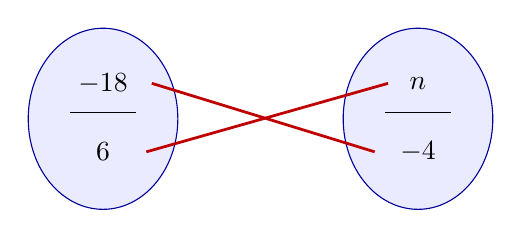
\begin{tikzpicture}[x=1cm,y=1cm]
  % left fraction inside its wing
  \fill[blue!8] (0,0) ellipse (0.95 and 1.15);
  \draw[blue!60!black] (0,0) ellipse (0.95 and 1.15);
  \node at (0,0.45) {$-18$};
  \draw (-0.42,0.08) -- (0.42,0.08);
  \node at (0,-0.42) {$6$};
  % right fraction inside its wing
  \fill[blue!8] (4,0) ellipse (0.95 and 1.15);
  \draw[blue!60!black] (4,0) ellipse (0.95 and 1.15);
  \node at (4,0.45) {$n$};
  \draw (3.58,0.08) -- (4.42,0.08);
  \node at (4,-0.42) {$-4$};
  % the two crossing diagonals
  \draw[red!75!black,line width=1pt] (0.62,0.45) -- (3.45,-0.42);
  \draw[red!75!black,line width=1pt] (0.55,-0.42) -- (3.62,0.45);
\end{tikzpicture}
\par\smallskip
Butterfly: multiply along each red line.
\end{center}

\begin{steps}[resume]
  \item Multiply along one red line: $(-18) \times (-4)$.
  \item Negative times negative is positive: $(-18) \times (-4) = 72$.
  \item Multiply along the other red line: $6 \times n = 6n$.
  \item Set the cross products equal: $6n = 72$.
  \item Divide both sides by 6 (same operation to both sides of the equals sign):
    \begin{center}
      $6n = 72$
      \par\smallskip
      $\underline{\div 6 \qquad \div 6}$
    \end{center}
  \item Simplify the left side: $6n \div 6 = n$. Dividing by 6 undoes the multiply-by-6.
  \item Now divide the right side: $72 \div 6$.
  \item Break 72 into $60 + 12$.
  \item Divide the first part: $60 \div 6 = 10$.
  \item Divide the second part: $12 \div 6 = 2$.
  \item Add the two quotients: $10 + 2 = 12$.
  \item So $n = 12$.
  \item Check the left fraction: $(-18) \div 6 = -3$.
  \item Check the right fraction: $12 \div (-4) = -3$.
  \item Both fractions equal $-3$, so the check works.
\end{steps}

\finalans{$n = 12$}

\blockhead{Why this makes sense}
\noindent Equal fractions have equal cross products. Both sides simplify to $-3$, so $n = 12$ is correct. A common mistake is mixing up which numbers multiply.
